%% Copyright (C) M. Giordano, O. Iovino, M. Leccardi, 2010-2013
%%
%% Quest'opera è distribuita con licenza Creative Commons,
%%  + Attribuzione
%%  + Non commerciale
%%  + Condividi allo stesso modo
%% 3.0 Italia.
%%
%% Il testo è disponibile alla pagina Internet
%% http://creativecommons.org/licenses/by-nc-sa/3.0/it

\documentclass[b5paper,11pt,oneside]{guidatematica}
\ProvidesFile{guidaemacsauctex.tex}[2013/01/08 v.0.0 Breve guida all'uso di
Emacs per LaTeX]

\usepackage{guidaemacsauctex}

\begin{document}

\frontmatter*

\title{Guida pratica all'uso\\ di\\ GNU Emacs \& AUCTeX}
\author{Mosè Giordano, Orlando Iovino, Matteo Leccardi}
\GetFileInfo{guidaemacsauctex.tex}
\date{\filename\ \fileversion\ del \filedate}
\maketitle

\chapter{Licenza d'uso}
\label{chap:licenza}

Quest'opera è soggetta alla Creative Commons Public License versione 3.0 o
posteriore: \emph{Attribuzione}, \emph{Non Commerciale}, \emph{Condividi allo
  stesso modo}. L'enunciato integrale della licenza è reperibile sul sito
ufficiale \url{http://creativecommons.org/licenses/by-nc-sa/3.0/deed.it}.

\bigskip\noindent\textsc{tu sei libero:}
\begin{itemize}
\item Di riprodurre, distribuire, comunicare al pubblico, esporre in pubblico,
      rappresentare, eseguire e recitare quest'opera.
\item Di modificare quest'opera.
\end{itemize}
\textsc{alle seguenti condizioni:}
\begin{itemize}
\item[\Large\ccAttribution] Devi attribuire la paternità dell'opera nei modi
      indicati dall'autore o da chi ti ha dato l'opera in licenza e in modo tale
      da non suggerire che essi avallino te o il modo in cui tu usi l'opera.
\item[\Large\ccNonCommercial] Non puoi usare quest'opera per fini commerciali.
\item[\Large\ccShareAlike] Se alteri o trasformi quest'opera, o se la usi per
      crearne un'altra, puoi distribuire l'opera risultante solo con una licenza
      identica o equivalente a questa.
\end{itemize}

\chapter{Presentazione}
\label{chap:presentazione}

Emacs è uno dei più vecchi e potenti editor di testo in circolazione e può
vantare fra i suoi utenti Donald Knuth (l'inventore di \TeX{}) e Laslie Lamport
(l'autore di \LaTeX{}).
% Fonti per Donald Knuth:
% https://www.informit.com/articles/article.aspx?p=1193856
% http://tex.loria.fr/litte/knuth-interview
% Fonte per Leslie Lamport:
% http://www.budiu.info/blog/2007/05/03/an-interview-with-leslie-lamport/
% Mihai Budui è un ricercatore della Microsoft
% (https://research.microsoft.com/en-us/people/mbudiu/), come Lamport, quindi
% l'intervista dovrebbe essere attendibile.
Questa guida tematica presenta il programma GNU Emacs ed il pacchetto \auctex{}
per i principali sistemi operativi: Windows, GNU/Linux e Mac OS. Dopo una
introduzione al programma, si spiega come installare (e configurare alcune
funzioni) \emacs{} e \auctex{} per scrivere documenti \LaTeX. Per finire si dà
qualche accenno per personalizzare e rendere più efficiente \emacs.

Si tenga presente che la guida è ben lontana dall'essere esauriente per un
editore di testi così importante come Emacs. Per ogni altro approfondimento non
riportato in queste righe rimandiamo il lettore ai manuali ufficiali, in
particolare a \cite{emacs:stallman} e \cite{auctex:manual}. Speriamo, con queste
brevi note, di convincere il lettore che Emacs non è poi così complicato come
spesso viene indicato.

Infine, qualche parola sulla composizione di questa guida tematica, scritta a
\emph{sei mani} grazie sistema di controllo di versione Git
(\url{http://git-scm.com}). Chi vuole collaborare può ``clonare'' il progetto
dal repository ufficiale presente sul sito \url{http://gitorious.org/} alla
pagina \url{https://gitorious.org/emacs-tutorial}. È inoltre gradita la
segnalazione di errori, refusi, commenti e suggerimenti o ogni altra forma di
collaborazione.

\begin{tabular}{cc}
\hspace{.32\textwidth} &                                                              \\
                       & \textsc{Mosè Giordano}                                       \\
                       & \textcolor{red}{\texttt{nome dot cognome at dominio dot it}} \\[0.5ex]
                       & \textsc{Orlando Iovino}                                      \\
                       & \texttt{orlando dot iovino at yahoo dot it}                  \\[0.5ex]
                       & \textsc{Matteo Leccardi}                                     \\
                       & \textcolor{red}{\texttt{nome dot cognome at dominio dot it}} \\
\end{tabular}

\newpage\tableofcontents*

\mainmatter

\chapter{Introduzione}
\label{chap:intro}

Lo sviluppo di \emacs{} è iniziato negli anni 1970 ai laboratori di Intelligenza
Artificiale del MIT, cioè molto prima che si diffondesse l'informatica che
conosciamo oggi.  Ciò comporta che \emacs{} utilizza una terminologia spesso
diversa da quella utilizzata dalla stragrande maggioranza degli altri programmi
che usiamo quotidianamente.  Per questo motivo non bisogna sorprendersi se
l'operazione di \emph{tagliare} del testo (generalmente indicata in inglese con
\emph{cutting}) in \emacs{} viene chiamata \emph{killing} e la successiva
operazione di \emph{incollare} il testo copiato (in inglese \emph{pasting})
viene chiamata \emph{yanking}.

\emacs{} è famoso per rendere possibile l'esecuzione di qualsiasi operazione
usando solo la tastiera, cioè senza l'ausilio del mouse.  A ogni comando può
essere associata una combinazione di tasti.  Sebbene questo fatto possa
inizialmente spaventare, è un vero punto di forza di \emacs{}, perché permette
di eseguire delle operazioni in maniera rapida, invece di dover spostare il
mouse alla ricerca di appositi bottoni.  In questa guida seguiremo la notazione
diffusa nel mondo di \emacs{} per indicare i tasti.  Quindi il tasto
\keys{\ctrl} verrà indicato con \verb!C!, l'\keys{Invio} viene indicato con
\verb!RET!, mentre \verb!M! indica il tasto \keys{\Meta}.  Sulle odierne
tastiere questo tasto è scomparso, si può ottenere lo stesso risultato con il
tasto \keys{\Alt} oppure premendo e rilasciando il tasto \keys{\esc}.  Nella
notazione di queste scorciatoie, un trattino fra due tasti all'interno di una
combinazione di tasti indica che i tasti vanno premuti contemporaneamente.
Così, quando si dirà che per eseguire un comando bisogna usare la combinazione
\verb!M-x! si dovranno premere contemporaneamente il tasto \keys{\Alt} e la
lettera \keys{x} oppure premere il tasto \keys{\esc}, rilasciarlo e premere la
lettera \keys{x}.

Il manuale di \emacs{}~\cite{emacs:stallman} può essere consultato all'interno
dello stesso editor di testo con le combinazioni di tasti \verb!C-h r!  (premere
contemporaneamente il tasto \keys{\ctrl} e la lettera \keys{h}, rilasciare
questi tasti e premere la lettera \keys{r}) oppure \verb!C-h i d m Emacs RET!
(premere contemporaneamente il tasto \keys{\ctrl} e la lettera \keys{h},
rilasciare questi tasti e premere la lettera \keys{i}, poi la lettera \keys{d},
poi la lettera \keys{m}, poi scrivere \verb!Emacs!  quindi premere il tasto
\keys{Invio}).  Se si preferisce, il manuale può anche essere consultato dal
menu \menu{Help > Read the Emacs Manual}.

Una delle caratteristiche principali di \emacs{} è che è un editor di testo
personalizzabile in ogni suo aspetto ed espandibile, in modo da renderlo adatto
alle proprie esigenze.  Il linguaggio utilizzato per espandere \emacs{} è
l'Elisp, un dialetto del Lisp sviluppato appositamente per \emacs{}.  Esistono
migliaia di pacchetti scritti in Emacs Lisp che permettono di estendere
ulteriormente le funzionalità di questo editor.

La versione standard di \emacs{}, senza pacchetti aggiuntivi, fornisce già un
discreto supporto alla creazione di documenti \LaTeX, ma il pacchetto \auctex{}
mette a disposizione numerosi strumenti che rendono senza alcun dubbio \emacs{}
uno degli editor di testo più potenti per la scrittura di documenti \LaTeX.  In
questa guida vedremo alcune delle funzioni principali di \auctex.

Per finire, prima di addentrarci nell'installazione di \emacs, \auctex{} e altri
programmi accessori, è utile riportare qui qualche indicazione sul file di
inizializzazione di \emacs, file che contiene codice Elisp per modificare il
comportamento delle funzioni.  Questo file ha diversi nomi e posti a seconda del
sistema operativo, in particolare
\begin{itemize}
\item Su Windows si chiama \filestyle{init.el} e va posizionato in
      \begin{itemize}
      \item \verb|C:\Documents and Settings\|\meta{nome
              utente}\verb|\Application\| fino ad XP;
      \item \verb|C:\Users\|\meta{nome utente}\verb|\AppData\.emacs.d\init.el|
            da Vista in avanti;
      \end{itemize}
\item Su GNU/Linux si chiama \filestyle{.emacs} o \filestyle{init.el} e va
      posizionato in \verb|~/.emacs|, \verb|~/.emacs.el| oppure
      \verb|~/.emacs.d/init.el|;
\item Su MAC OS \textcolor{red}{[\ldots]}
\end{itemize}
Nel seguito ci riferiremo spesso al file di inizializzazione chiamandolo
semplicemente \verb|.emacs|, indipendentemente dalla posizione in cui si trova e
dall'effettivo nome utilizzato nel proprio sistema (\verb|.emacs|,
\verb|.emacs.el| oppure \verb|init.el|).

%% --------------------------------------------------------------------------
%% Windows
%% --------------------------------------------------------------------------


\chapter{Emacs e AUC\TeX{}  su Windows}
\label{oi:chap:windows}

\epigraph{(\textit{a cura di} Orlando Iovino)}

\section{Installare Emacs}
\label{oi:sec:installemacs}

Per sistemi operativi Microsoft Windows non esiste una vera e propria procedura
di installazione. \emacs{} si può utilizzare semplicemente procurandosi
l'archivio che contiene gli eseguibili.

All'indirizzo \url{http://ftp.gnu.org/pub/gnu/emacs/windows/} si scarica
l'archivio compresso \filestyle{emacs-24.2-bin-i386.zip} e lo si decomprime in
una posizione di comodo; una buona soluzione, per esempio, è decomprimere il
suddetto archivio in \directory{C:/Programmi/Emacs/} che assumeremo, da questo
momento, come cartella di installazione.

Se si vuole creare un collegamento di \emacs{} nel menù Start, è sufficiente
eseguire il programma \progstyle{addpm.exe} contenuto nella cartella
\directory{C:/Programmi/Emacs/bin}.

A questo punto \emacs{} è pronto per scrivere documenti in \LaTeX: l'utente
infatti non deve specificare nessun percorso circa gli eseguibili della
distribuzione \LaTeX\ installata perché \emacs{} li trova da solo.

\section{Installare AUC\TeX}
\label{oi:sec:installauctex}

Si scarica l'archivio compresso \filestyle{auctex-11.87-e24.2-msw.zip}
dall'indirizzo \url{http://www.gnu.org/software/auctex/download-for-windows} e
lo si decomprime in \directory{C:/Programmi/Emacs/}.  Si noti che alcuni file
sono gli stessi, perciò basta unire il contenuto dell'archivio di \auctex{} con
quello di \emacs.

Dopo aver installato \auctex, \emacs{} caricherà da solo i file necessari per
attivare la modalità \verb!latex-mode!, propria di \auctex, quando si apre e/o
crea un file con estensione \filestyle{.tex}.

\section{Correttore ortografico}
\label{oi:sec:aspell}

Per usare il correttore ortografico in \emacs{} si deve installare il programma
\progstyle{GNU Aspell} disponibile all'indirizzo
\url{http://aspell.net/win32/}. L'ultima versione stabile è la 0.50-3 datata
Dicembre 2002.

Si devono installare, nell'ordine
\begin{enumerate}
\item il programma \progstyle{Aspell-0-50-3-3-Setup.exe};
\item il dizionario precompilato per l'italiano \progstyle{Aspell-it-0.50-2-3.exe}.
\end{enumerate}

Resta qualche altra operazione da fare. Come prima cosa si deve copiare il
percorso della cartella dove sono contenuti gli eseguibili di \progstyle{Aspell}
nella variabile d'ambiente \textsf{PATH}. Secondo, aggiungere al proprio file
\filestyle{.init} le seguenti righe:
\begin{lstlisting}
(setq-default ispell-program-name "aspell")
(setq-default ispell-extra-args '("--reverse"))
(setq ispell-dictionary "italiano")
\end{lstlisting}
dove, la prima e la terza sono quelle strettamente necessarie, mentre la seconda
riga serve a risolvere dei problemi con le versioni precedenti di \emacs.

\section{Ricerca diretta inversa}
\label{oi:sec:ricdirinv}

Prima di attivare la ricerca diretta inversa, si spiega come risolvere il
problema dei diritti di amministratore --- qualora l'account utente ne sia
fornito ---, per sistemi operativi Vista e Seven (su Xp non dovrebbero esserci
problemi, per Windows 8 non è stato possibile provarlo). Infatti, in tale
situazione è possibile avere problemi con la cartella \emph{server} del tipo
\begin{lstlisting}[keywordstyle=\color{black}]
error: The directory '~/.emacs.d/server' is unsafe
\end{lstlisting}

Una possibile soluzione, riportata in~\cite{setupwindows}, è la seguente. Si
deve aprire il prompt dei comandi e portarsi nella cartella che contiene, a sua
volta, la cartella \emph{server} scrivendo nella riga di comando un'istruzione
del tipo
\begin{lstlisting}[language=bash]
cd C:/Users/£\meta{nome utente}£/Roaming/.emacs.d
\end{lstlisting}
oppure
\begin{lstlisting}[language=bash]
cd %APPDATA%/.emacs.d
\end{lstlisting}
ed infine
\begin{lstlisting}
takeown /f server
\end{lstlisting}
Se l'operazione sarà andata a buon fine verrà segnalato con qualcosa come
\begin{lstlisting}
OPERAZIONE RIUSCITA: il file o la cartella ...
\end{lstlisting}

Si può ora configurare \emacs{} per la ricerca diretta inversa con il
visualizzatore \progstyle{SumatraPDF} --- l'unico in grado di supportare questa
funzione in sistemi Windows ---, che si scarica dal sito
\url{http://blog.kowalczyk.info/software/sumatrapdf/free-pdf-reader.html}.

Per la ricerca diretta basta scrivere nel file di inizializzazione
\filestyle{.init} il codice
\begin{lstlisting}
(setq TeX-source-correlate-method (quote synctex))
(setq TeX-source-correlate-mode t)
(setq TeX-source-correlate-start-server t)

(setq TeX-view-program-list
      '(("Sumatra PDF" ("\"C:/Program Files (x86)/SumatraPDF/SumatraPDF.exe\" -reuse-instance"
	  (mode-io-correlate " -forward-search %b %n") " %o"))))

(setq TeX-view-program-selection
      '(((output-dvi style-pstricks) "dvips and start")
	(output-dvi "Yap")
	(output-pdf "Sumatra PDF")
	(output-html "start")))
\end{lstlisting}
invece, per la ricerca inversa si deve aprire \progstyle{SumatraPDF}, andare nel
menu \emph{Impostazioni}, quindi scegliere \emph{Opzioni...} e scrivere
\begin{lstlisting}[flexiblecolumns]
C:/Programmi/Emacs/bin/emacsclientw.exe --no-wait +%l "%f"
\end{lstlisting}
in \emph{Imposta la ricerca inversa via riga di comando}, come si vede dalla
figura~\ref{oi:fig:sumatra:setup}.
\begin{figure}[t]
  \centering
  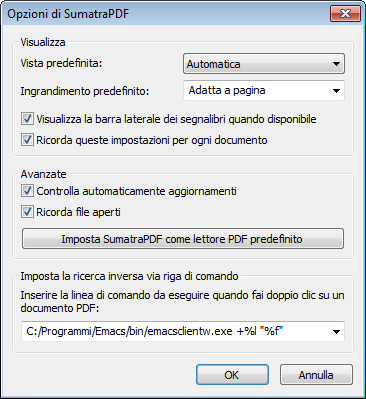
\includegraphics[width=0.50\textwidth]{sumatrapdf}
  \caption{Impostazioni per il visualizzatore SumatraPDF.}
  \label{oi:fig:sumatra:setup}
\end{figure}

Si faccia attenzione quando si copia e incolla il codice da questo documento:
potrebbe essere necessario riscrivere i caratteri \verb|"| e \verb|'| in
\emacs. Inoltre il codice in cui si modificano le variabili
\verb!TeX-view-program-list! e \verb!TeX-view-program-selection! è qui spezzato
in più righe per una questione di praticità, ma dovrebbe essere scritto su
un'unica riga per ognuna della variabili.

Con queste impostazioni il visualizzatore predefinito per \emacs\ -- non del
sistema operativo -- sarà \progstyle{SumatraPDF}. Per usare la ricerca diretta
si devono premere i tasti \verb!C-c C-v! ed il visualizzatore si aprirà/porterà
in corrispondenza della riga di \emacs{} in cui è il cursore. Per la ricerca
inversa basta invece un doppio clic nel visualizzatore.

%% --------------------------------------------------------------------------
%% GNU/Linux
%% --------------------------------------------------------------------------

\chapter{Emacs e AUC\TeX{} su GNU/Linux}
\label{mg:chap:linux}

\epigraph{(\textit{a cura di} Mosè Giordano)}

\section{Installare Emacs}
\label{mg:sec:installemacs}

\emacs{} fa parte del progetto GNU quindi è presente in tutti i
sistemi operativi della famiglia GNU/Linux. Se non è già installato,
il metodo più semplice per ottenere \emacs{} in un sistema GNU/Linux è
far riferimento al gestore pacchetti della propria distribuzione. Si
possono naturalmente utilizzare i gestori di pacchetti a interfaccia
grafica, riportiamo qui inoltre i comandi da terminale che possono
essere eseguiti per installare \emacs{} in alcune delle principali
distribuzioni: Debian e Ubuntu:
\begin{lstlisting}
$ sudo apt-get install emacs
\end{lstlisting}
Fedora:
\begin{lstlisting}
$ sudo yum install emacs
\end{lstlisting}
OpenSUSE:
\begin{lstlisting}
$ sudo zypper install emacs
\end{lstlisting}

Il metodo più difficile, per i non avvezzi all'uso del terminale,
consiste nel compilare \emacs{} a partire dal codice sorgente,
tuttavia non è intenzione di questa guida spiegare come fare ciò.

Dopo averlo installato, \emacs{} potrà essere avviato facendo clic sul
suo lanciatore oppure eseguendo da terminale il comando
\begin{lstlisting}
$ emacs
\end{lstlisting}
Se si desidera utilizzare \emacs{} con interfaccia testuale bisogna
aggiungere l'opzione \texttt{-nw} oppure \texttt{--no-window-system}:
\begin{lstlisting}
$ emacs -nw
\end{lstlisting}
Possono essere aggiunti come argomenti da linea di comando il percorso
del file (o dei file) che si vogliono modificare:
\begin{lstlisting}
$ emacs file1.tex file2.tex
\end{lstlisting}

\section{Installare AUC\TeX}
\label{mg:sec:installauctex}

Anche il pacchetto \auctex{} è presente nei sistemi GNU/Linux. Come già detto
per \emacs, per installare \auctex{} si consiglia di utilizzare il gestore
pacchetti della propria distribuzione. Ecco i comandi da usare per installare da
terminale il pacchetto nelle principali distribuzioni: Debian e Ubuntu:
\begin{lstlisting}
$ sudo apt-get install auctex
\end{lstlisting}
Fedora:
\begin{lstlisting}
$ sudo yum install emacs-auctex
\end{lstlisting}
OpenSUSE:
\begin{lstlisting}
$ sudo zypper install emacs-auctex
\end{lstlisting}

Su Debian e Ubuntu potrebbe essere raccomandata l'installazione della
distribuzione TeX Live presente nei repository ufficiali del sistema operativo.
Per evitare che questo avvenga, per esempio perché si utilizza una distribuzione
TeX Live installata in altro modo, se si installa il pacchetto da terminale è
sufficiente aggiungere l'opzione \verb!--no-install-recommends!
\begin{lstlisting}
$ sudo apt-get install --no-install-recommends auctex
\end{lstlisting}

\section{Correttore ortografico}
\label{mg:sec:aspell}

Il correttore ortografico GNU Aspell può essere installato facilmente
su GNU/Linux utilizzando, come al solito, il gestore pacchetti della
propria distribuzione. Il dizionario italiano di GNU Aspell si chiama
\texttt{aspell-it} quindi da terminale può essere installato in Debian
con il comando
\begin{lstlisting}
$ sudo apt-get install aspell-it
\end{lstlisting}
in Fedora con
\begin{lstlisting}
$ sudo yum install aspell-it
\end{lstlisting}
mentre in openSUSE si può eseguire il comando:
\begin{lstlisting}
$ sudo zypper install aspell-it
\end{lstlisting}


%% --------------------------------------------------------------------------
%% Mac OS
%% --------------------------------------------------------------------------

\chapter{Emacs e AUC\TeX{} su Mac OS}
\label{ml:chap:linux}

\epigraph{(\textit{a cura di} Matteo Leccardi)}

\section{Installare Emacs}
\label{ml:sec:installemacs}

Sul mirror ufficiale \url{http://ftp.gnu.org/pub/gnu/emacs/} non
è presente una versione già compilata per Mac OS X, queste versioni
sono rese disponibili da vari volontari come ad esempio il gestore del
sito \url{http://emacsformacosx.com/}. La
procedura per l'installazione è quella consueta: scaricata la versione
più recente si apre il file dmg (se non è già stato aperto
automaticamente al termine del download) e si trascina Emacs nella
cartella Applicazioni.

In Mac OS le applicazioni avviate dall'interfaccia grafica non hanno
accesso ai valori delle variabili d'ambiente, per rendere disponibile
ad \emacs{} la variabile \texttt{PATH} è necessario dare da terminale
il comando
\begin{lstlisting}
$ defaults write ~/.MacOSX/environment PATH "$PATH"
\end{lstlisting}
Le nuove impostazioni sono effettive dopo aver eseguito un logout e un
successivo login.

Il comando va ripetuto ogni volta che si installa qualche programma
che modifica il valore di \texttt{PATH}, il caso che più probabilmente
riguarda i lettori di questa guida è la distribuzione \TeX{}.

% TODO: controllare che i tasti inseriti con `\keys{}' siano corretti
Per gli utenti che usano la tastiera italiana è utile impostare il
tasto \keys{\cmdmac} come \keys{\Meta} e il tasto \keys{\Altmac} per
scrivere i caratteri speciali, in particolare le parentesi quadre, le
graffe e la tilde, scrivendo queste righe nel file \filestyle{.emacs}
\begin{lstlisting}
(setq ns-command-modifier 'meta)
(setq ns-alternate-modifier nil)
\end{lstlisting}

\section{Installare AUC\TeX}
\label{ml:sec:installauctex}

Come per \emacs{} non è disponibile una versione di \auctex{} già compilata per
Mac OS, in questo caso non esistono neppure versioni non ufficiali ed è quindi
necessario utilizzare il programma \progstyle{make}.  \progstyle{make} viene
installato insieme all'ambiente di sviluppo
\href{http://developer.apple.com/technologies/tools/whats-new.html}%
{\progstyle{Xcode}}. Chi non intende dedicare svariati GB di disco a un software
utile soltanto a chi sviluppa software può sfruttare il fatto che
\progstyle{make} viene installato anche dal correttore ortografico
\progstyle{cocoAspell} la cui installazione è descritta nel
paragrafo~\ref{ml:sec:aspell}.

Dalla pagina relativa a Mac OS X,
\url{http://www.gnu.org/software/auctex/download-for-macosx.html} bisogna
scaricare l'archivio compresso \filestyle{auctex-11.87.tar.gz}.

Dopo aver estratto il contenuto dell'archivio in una cartella temporanea occorre
aprire una sessione di terminale e portarsi nella cartella appena creata.

Configurare \auctex{} con il comando
\begin{lstlisting}[flexiblecolumns]
$ ./configure \
 --prefix=/Applications/Emacs.app/Contents/Resources/ \
 --with-emacs=/Applications/Emacs.app/Contents/MacOS/Emacs \
 --with-lispdir=/Applications/Emacs.app/Contents/Resources \
                  /site-lisp/ \
 --without-texmf-dir
\end{lstlisting}
sostituendo se necessario a \texttt{Applications}\footnote{Utilizzando il
  terminale non bisogna utilizzare i nomi localizzati delle cartelle ma quelli
  reali, quindi \texttt{Application} è corretto anche se si utilizza la versione
  italiana di Mac OS.} la cartella in cui si trova \emacs{}, in questo modo tutti
i file saranno contenuti nel bundle \texttt{Emacs.app}.

Compilare e installare con il comando
\begin{lstlisting}
$ make && make install
\end{lstlisting}

Dopo l'installazione bisogna impostare i visualizzatori per i vari file creati
con \LaTeX{} scrivendo nel file \filestyle{.emacs} queste righe
\begin{lstlisting}
(setq TeX-view-program-list
      '(("dvips and Skim" "%(o?)dvips %d -o &&\
  /Applications/Skim.app/Contents/SharedSupport/\
displayline %n %f %b")
	("Skim" "/Applications/Skim.app/Contents/\
SharedSupport/displayline %n %o %b")
        ("open" "open %o")))
(setq TeX-view-program-selection
      '(((output-dvi style-pstricks) "dvips and Skim")
        (output-dvi "Skim")
        (output-pdf "Skim")
        (output-html "open")))
\end{lstlisting}
Come visualizzatore si usa \progstyle{Skim},
\url{http://skim-app.sourceforge.net/}, perché supporta la ricerca diretta e
inversa dal \filestyle{pdf}, i dettagli sulla configurazione di \emacs{} e
\progstyle{Skim} sono riportati nel paragrafo~\ref{ml:sec:ricdirinv}.

\section{Correttore ortografico}
\label{ml:sec:aspell}

Anche per Mac OS X è disponibile una versione di \progstyle{GNU Aspell} chiamata
\progstyle{cocoAspell}, disponibile all'indirizzo
\url{http://cocoaspell.leuski.net/}.

Dopo aver installato la versione 2.1 (ad oggi l'ultima versione) si possono
installare i dizionari delle lingue che interessano scaricandoli direttamente
dal sito di \progstyle{GNU Aspell}, all'indirizzo
\url{ftp://ftp.gnu.org/gnu/aspell/dict/}, ad esempio il dizionario italiano è
contenuto nell'archivio
\href{ftp://ftp.gnu.org/gnu/aspell/dict/it/aspell6-it-2.2_20050523-0.tar.bz2}%
{\filestyle{aspell6-it-2.2\_20050523-0.tar.bz2}}.

Dopo aver scaricato i dizionari bisogna estrarre il contento
dell'archivio in una cartella temporanea, aprire una sessione di
terminale e portarsi nella cartella appena creata. I dizionari si
installano dando i seguenti comandi
\begin{lstlisting}
$ ./configure
$ make
$ sudo make install
\end{lstlisting}

Come ultima cosa è necessario configurare \emacs\ aggiungendo al
\filestyle{.emacs} le seguenti righe:
\begin{lstlisting}
(setq-default ispell-program-name "aspell")
(setq ispell-dictionary "italiano")
\end{lstlisting}

\section{Ricerca diretta inversa}
\label{ml:sec:ricdirinv}

L'unico visualizzatore di file \filestyle{pdf} per Mac OS X che supporta la
ricerca diretta e inversa associato a \emacs{} è
\href{http://skim-app.sourceforge.net/}{\progstyle{Skim}}, già citato nel
paragrafo~\ref{ml:sec:installauctex}, relativo all'installazione di
\auctex{}.

Dopo averlo installato occorre configurarlo impostando quanto segue
nella pagina \emph{Sincronizza} delle preferenze:
\begin{itemize}
\item selezionare la checkbox \emph{Controlla cambiamenti del file}
\item nel campo \emph{Comando} scrivere \\
      \verb!/Applications/Emacs.app/Contents/MacOS/bin/emacsclient!
\item scrivere \verb!--no-wait +%line "%file"! nel campo
      \emph{Argomenti}
\end{itemize}
Nella figura~\ref{fig:skimpref} sono riportate le impostazioni
corrette.
\begin{figure}[tb]
  \centering
  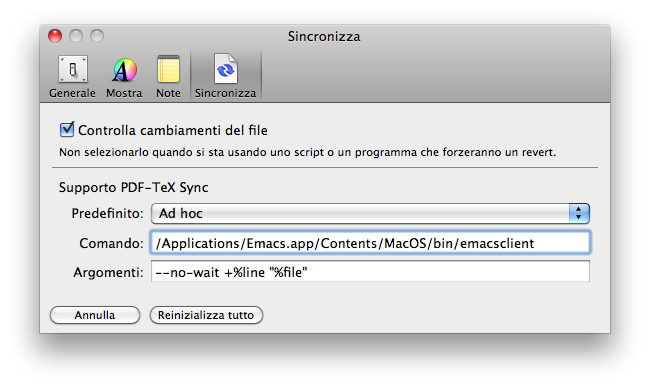
\includegraphics[width=\textwidth]{preferenze_skim}
  \caption{Preferenze di Skim per la ricerca diretta e inversa}
  \label{fig:skimpref}
\end{figure}

La prima opzione fa sì che quando un file aperto in \progstyle{Skim} viene
modificato da un altro processo \progstyle{Skim} chieda se deve essere
ricaricato, scegliendo Automatico successivi aggiornamenti vengono ricaricati
senza chiedere conferma.

La configurazione di \emacs{} è analoga a quella degli altri sistemi
operativi, occorre scrivere queste righe in \filestyle{.emacs}
\begin{lstlisting}
(setq TeX-source-correlate-method 'synctex)
(setq TeX-source-correlate-mode t)
(setq TeX-source-correlate-start-server t)
\end{lstlisting}

Per passare dal file \filestyle{.tex} al \filestyle{.pdf} si utilizza la
combinazione di tasti \verb!C-c C-v!, per ritornare al file \filestyle{.tex}
bisogna fare click sulla parola che interessa tendendo premuto \keys{\shift} e
\keys{cmd}.

Con alcune versioni di \emacs{} precedenti alla 23.3 resta in primo
piano la finestra del visualizzatore, in tal caso è necessario
aggiungere queste righe al file \filestyle{.emacs}
\begin{lstlisting}
(defun ns-raise-emacs ()
  (ns-do-applescript "tell application \"Emacs\" to activate"))
(add-hook 'server-switch-hook 'ns-raise-emacs)
\end{lstlisting}

\chapter{Primi passi in \emacs}
\label{chap:primi-passi-emacs}

Nei precedenti capitoli si è in sostanza parlato di come installare e
configurare i principali componenti per scrivere documenti in \LaTeX\ con
\emacs. In questo capitolo vediamo ora come si scrive in \emacs un documento
\filestyle{.tex}.

\section{Ciao mondo}
\label{sec:primodocumento}

Su ogni sistema operativo si ha la possibilità di aprire \emacs\ a partire da un
collegamento al programma principale. Aperto \emacs, si dovrebbe avere davanti
la finestra principale, come in figura~\ref{fig:principale}.

\begin{figure}[ht]
  \centering
  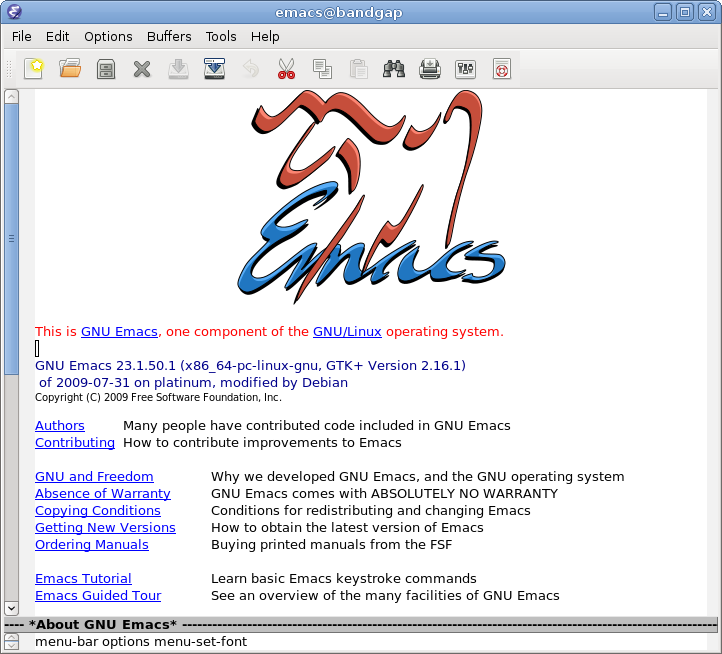
\includegraphics[width=\textwidth]{splash}
  \caption{Schermata iniziale di GNU Emacs. L'immagine è presa dal sito
    ufficiale \url{http://www.gnu.org/software/emacs/}.}
  \label{fig:principale}
\end{figure}

Per creare un nuovo documento ci sono due modi: si può andare nel menu
\menu{File > Visit New File...} oppure basta premere \verb|C-x C-f| ed Emacs
chiederà di aprire/trovare un file. Scrivendo un nome che nella cartella di
lavoro non esiste questo file sarà creato. Scritto il nome del file, per esempio
\filestyle{primo.tex}, si può iniziare a scrivere in \LaTeX. Per gli amanti
delle scorciatoie da tastiera (e di questo \emacs\ ne fa un suo punto di forza),
scrivendo \verb|C-c C-e|, \emacs\ chiederà quale ambiente inserire; dato che a
questo punto non c'è alcun documento attivo, l'ambiente \ambstyle{document} sarà
proposto come quello predefinito
\begin{lstlisting}
Environment type: (default document) 
\end{lstlisting}
Dopo il primo \verb|RET| apparirà nel minibuffer la scritta
\begin{lstlisting}
Document class: (default article) 
\end{lstlisting}
in cui si può scegliere la classe che, per impostazione predefinita, è
\classstyle{article}. A seguito del secondo \verb|RET| si avrà
\begin{lstlisting}
Options: 
\end{lstlisting}
in cui scrivere le opzioni della classe. Scelte queste ultime si darà un altro
\verb|RET| e si avrà infine il classico
\begin{lstlisting}[language={[LaTeX]TeX}]
\documentclass{article}

\begin{document}
£\meta{\textrm{cursore del mouse}}£
\end{document}
\end{lstlisting}
con il cursore posizionato nell'ambiente \ambstyle{document}.

Scritto quello che si vuole nel documento, per compilarlo si può
\begin{compactitemize}
\item premere sul pulsante presente nella \emph{toolbar}
\item andare in \menu{Command > LaTeX}
\item scrivere \verb|C-c C-c|. Solo in questo caso nel minibuffer si avrà
\begin{lstlisting}
Command: (default LaTeX)
\end{lstlisting}
      e premendo \verb|RET| sarà lanciato \LaTeX.
\end{compactitemize}
Durante la compilazione del documento uscirà
\begin{lstlisting}
Type `C-c C-l' to display results of compilation.
\end{lstlisting}
e al termine, invece, se tutto è andato a buon fine senza errori, si avrà
\begin{lstlisting}
LaTeX: successfully formatted {1} page
\end{lstlisting}
Con questa procedura si scrive un nuovo documento in \LaTeX. 

Senza nessuna personale impostazione, con il procedimento di cui sopra viene
creato un file \filestyle{.dvi}. Se si vuole creare un file \filestyle{.pdf} con
gli stessi comandi accennati, si deve scrivere
\begin{lstlisting}
(add-hook 'LaTeX-mode-hook 'TeX-PDF-mode)
\end{lstlisting}
nel file \filestyle{.emacs}.

Per visualizzare il documento prodotto, sia esso un file \filestyle{.dvi} o un
\filestyle{.pdf}, si può
\begin{compactitemize}
\item premere sul pulsante presente nella \emph{toolbar}
\item andare in \menu{Command > View} e dare poi \verb|RET|
\item scrivere \verb|C-c C-C RET| o \verb|C-c C-v|.
\end{compactitemize}
In tutti e tre i casi, se \emacs\ e \auctex\ sono configurati per lavorare con
ricerca diretta-inversa, il visualizzatore dovrebbe aprirsi sulla riga
corrispondente del file sorgente.

\section{Un documento più complesso}
\label{sec:documento:complesso}

Per documenti abbastanza corposi, come un libro, un manuale, una tesi \ldots,
conviente suddividere il documento in un file principale, che chiameremo per
esempio \filestyle{master.tex}, e altri file contenenti il materiale vero e
proprio, ad esempio \filestyle{capitolouno.tex} e \filestyle{capitolodue.tex}.

\emacs, come diversi altri editor di testo, consente di lanciare la compilazione
direttamente dal file su cui si sta lavorando anche se questo non è il file
principale, cioè il file \filestyle{master.tex} che conterrà qualcosa come
\begin{lstlisting}[language={[LaTeX]TeX}]
\documentclass{book}

\begin{document}

\input{capitolouno}
\input{capitolodue}

\end{document}

%%% Local Variables: 
%%% mode: latex
%%% TeX-master: t
%%% End: 
\end{lstlisting}

Si nota subito una cosa non presente nel file del
paragrafo~\ref{sec:primodocumento}: le varibili locali.

Le variabili locali sono dei meta commenti che \LaTeX\ ignora --- in quanto
commenti ---, ma \emacs\ no e che servono per impostare alcune preferenze sul
proprio documento.

Le variabili locali si possono specificare tra \verb|%%% Local Variables:| e
\verb|%%% End:| alla fine del file oppure tra \verb|-*-| e \verb|-*-| all'inizio
del file. Riferiamoci al primo caso.

Prima di andare avanti è bene anche specificare che le variabili di cui
parleremo sono però messe a disposizone di \auctex. La riga
\verb|%%% mode: latex| indica che
stiamo scrivendo un documento \LaTeX, mentre \verb|TeX-master: t| indica che il
file in questione è il file principale su cui lanciare le compilazioni.

I file \filestyle{capitolouno.tex} e \filestyle{capitolodue.tex}, oltre al
proprio contenuto, conterrano invece alla fine le righe
\begin{lstlisting}[language={[LaTeX]TeX}]
%%% Local Variables: 
%%% mode: latex
%%% TeX-master: "master"
%%% End: 
\end{lstlisting}
in cui si specifica che la compilazione debba essere lanciata sul file
\filestyle{master.tex} mediante la riga \verb|%%% TeX-master: "master"|.

Per fare in modo che all'apertura di un nuovo documento sia chiesto se il file
debba essere o meno un file \emph{master}, si deve scrivere 
\begin{lstlisting}
(setq-default TeX-master nil)
\end{lstlisting}
nel file \filestyle{.emacs}, come specificato anche nel
capitolo~\ref{chap:personal}.

\section{Correzione ortografica}
\label{sec:corr:orto:in:azione}

Viste le modalità di installazione dei correttori ortografici specifichiamo in
questo paragrafo come usarli, indipendentemente dal sistema oprativo.

Per fare una revisione del documento che si sta scrivendo, bisogna premere la
combinazione di tasti \verb!M-x! e scrivere \verb!ispell!: in questo modo il
dizionario proporrà, in sequenza, la correzione dei termini che trova errati.

Un secondo modo, per scrivere correttamente, è attivare la modalità
\emph{flyspell} (correzione al volo). Se la si vuole attivare solo sul documento
corrente basta andare in \menu{Tools > Spell Checking > Automatic spell checking
  (Flyspell)}; se invece la si vuole tenere sempre abilitata si deve aggiungere
la riga:
\begin{lstlisting}
(add-hook 'LaTeX-mode-hook 'flyspell-mode)
\end{lstlisting}
al proprio file \filestyle{.emacs}.

Quando viene rilevata una parola potenzialmente non corretta, questa verrà
colorata (in genere) in rosso. Alcuni termini, però, vengono segnalati come
errati anche quando sono corretti, cosa che accade perché quel termine non è
presente nel dizionario: si può aggiungerlo, premendo il tasto centrale del
mouse quando questo è posizionato sulla parola e scegliere \texttt{Save word}.

\section{Sinossi delle principali scorciatoie}
\label{sec:sinossi:sco}

\emacs\ gode di una infinità di combinazioni di tasti per eseguire operazioni
banali e non. Scriverle tutte sarabbe impossibile. Va da sé che per usare \emacs
non è necessario ricordarle tutte ma almeno le principale sì, anche se con l'uso
quotidiano, queste ultime si memorizzano automaticamente. Le principali sono qui
riassunte nella tabella~\ref{tab:cheat-sheet}. Pur essendo abbastanza corposa,
la tabella comunque non ricopre tutte le possibili combinazioni. Quelle
strettamente necessarie sono le prime. Per approfondire il discorso si possono
anche consultare le \emph{Reference Card}, disponibili in genere nella propria
installazione.

\begin{longtable}{>{\ttfamily}l>{\ttfamily}lp{0.32\textwidth}}
  % intestazione iniziale
  \caption{Scorciatoia è la combinazione di tasti da premere per ottenere il
    risultato descritto nell'ultima colonna.  La seconda colonna riporta la
    funzione, da eseguire con \texttt{M-x}, a cui è legata quella combinazione
    di tasti.}
  \label{tab:cheat-sheet} \\
  \toprule
  {\normalfont\scshape Scorciatoia} & {\normalfont\scshape Funzione} &
  \textsc{Effetto} \\
  \midrule
  \endfirsthead
  % intestazione normale
  \multicolumn{3}{l}{\footnotesize\itshape
    Continua dalla pagina precedente} \\
  \toprule
  {\normalfont\scshape Scorciatoia} & {\normalfont\scshape Funzione} &
  \textsc{Effetto} \\
  \midrule
  \endhead
  % piede normale
  \midrule
  \multicolumn{3}{r}{\footnotesize\itshape
    Continua nella prossima pagina} \\
  \endfoot
  % piede finale
  \bottomrule
  \multicolumn{3}{r}{\footnotesize\itshape
    Si conclude dalla pagina precedente} \\
  \endlastfoot
  % corpo della tabella
  C-x C-f & find-file & Apre il file da specificare nel minibuffer \\
  C-x C-s & save-buffer & Salva il buffer attuale \\
  C-x C-w & write-file & Salva il file attuale nel file indicato nel minibuffer
  \\
  C-x C-c & - & Chiede se salvare i buffer aperti e
  chiude Emacs \\
  C-g & keyboard-quit & Interrompe il comando in esecuzione \\
  C-x u & undo & Annulla l'ultima operazione \\
  \midrule
  \multicolumn{3}{c}{Ricerca e sostituisci} \\
  \midrule
  C-s & isearch-forward & Ricerca incrementale in avanti \\
  C-r & isearch-backward & Ricerca incrementale indietro \\
  M-g g & goto-line & Sposta il cursore alla riga specificata nel minibuffer \\
  M-\% & query-replace & Ricerca e sostituzione \\
  \midrule
  \multicolumn{3}{c}{Copia e incolla} \\
  \midrule
  M-w & kill-ring-save & Copia la regione selezionata \\
  C-y & yank & Incolla l'ultima selezione \\
  C-w & kill-region & Taglia la regione selezionata \\
  C-k & kill-line & Taglia il resto della riga attuale \\
  \midrule
  \multicolumn{3}{c}{Aiuto} \\
  \midrule
  C-h ? & help-for-help & Apre una finestra di aiuto \\
  C-h k & describe-key & Mostra la documentazione della combinazione di tasti
  che viene successivamente premuta \\
  C-h f & describe-function & Mostra la documentazione della funzione
  specificata nel minibuffer \\
  \midrule
  \multicolumn{3}{c}{Navigazione fra i buffer} \\
  \midrule
  C-x b & switch-to-buffer & Cambia buffer visualizzato \\
  C-x C-b & list-buffers & Mostra l'elenco dei buffer \\
  C-x k & kill-buffer & Chiude il buffer specificato nel minibuffer \\
  \midrule
  \multicolumn{3}{c}{``Window''} \\
  \midrule
  C-x 2 & - & Divide la ``window'' attuale in due, verticalmente \\
  C-x 3 & - & Divide la ``window'' attuale in due, orizzontalmente \\
  C-x o & other-window & Sposta il cursore nella ``window'' successiva \\
  C-x 0 & delete-window & Chiude la ``window'' attuale \\
  C-x 1 & - & Chiude tutte le ``windows'' tranne quella attuale \\
\end{longtable}

\chapter{Personalizzare \emacs{} \& \auctex}
\label{chap:personal}

In questo capitolo vedremo alcune delle personalizzazioni che possono risultare
utili quando si lavora con documenti \LaTeX{}.  Per modificare le impostazioni
relative alla gestione nativa di \TeX{} da parte di \emacs{} è possibile usare
la funzione \verb!M-x customize-group RET tex RET!.  In questo modo si aprirà un
buffer nel quale sarà possibile modificare, tramite l'interfaccia, le opzioni
desiderate.  Per modificare in particolare \auctex{} è possibile usare la
funzione \verb!M-x customize-group RET AUCTeX RET!.

Di seguito saranno suggerite alcune porzioni di codice Elisp che permettono di
personalizzare \emacs{} e che vanno inserite nel file di inizializzazione
\filestyle{.emacs}.  Per rendere effettive le modifiche bisogna riavviare
\emacs{}.

Se si usa \auctex{}, è possibile inserire macro nei propri documenti \LaTeX{}
con \verb!C-c RET!.  La comodità di questa funzione è che \auctex{} conosce le
macro dei principali pacchetti \LaTeX{} e permette quindi l'autocompletamento
con il tasto TAB.  Inoltre conosce gli argomenti e le opzioni che queste macro
accettano, infatti usando \verb!C-c RET frac RET! nel documento si otterrà
\verb!\frac{}{}!  e il cursore si posizionerà all'interno del primo paio di
parentesi graffe.  Allo stesso modo, usando \verb!C-c RET sqrt RET! verrà
richiesto l'ordine \verb!n! della radice da inserire (premere direttamente
\verb!RET! per non inserire nulla) e si otterrà \verb!\sqrt[n]{}!.  Per fare in
modo che \auctex{} conosca quali pacchetti \LaTeX{} sono stati caricati bisogna
permettergli di effettuare il parsing dei propri documenti e questo è possibile
aggiungendo nel proprio file \filestyle{.emacs} il seguente codice
\begin{lstlisting}
(setq TeX-parse-self t) ; Attiva parsing al caricamento
(setq TeX-auto-save  t) ; Attiva parsing al salvataggio
\end{lstlisting}
In questo modo verrà creata una cartella chiamata \verb!auto! nella stessa
cartella in cui si trova il documento nella quale verranno registrate le
informazioni relative al proprio documento \LaTeX{}, se non si desidera
affollamento nelle proprie cartelle si potrebbe non voler attivare queste due
opzioni.

Come detto, \auctex{} conosce le macro dei pacchetti principali, ma naturalmente
non conosce tutte i pacchetti.  Si può far in modo che \auctex{} analizzi tutti
i file di stile della propria distribuzione \LaTeX{} eseguendo il comando
\verb!M-x TeX-auto-generate-global!.  In questo modo verrà automaticamente
aggiunto il supporto a tutti i pacchetti, almeno quelli non troppo complicati e
che non siano basati su \LaTeX{}3.  L'operazione può richiedere alcuni minuti,
soprattutto la prima volta che viene eseguito.  Per i pacchetti non
correttamente analizzati da \auctex{}, possiamo aggiungere manualmente le macro
da utilizzare solo quando viene caricato nel documento \LaTeX{} il pacchetto che
fornisce le relative macro.  Per esempio, uno dei pacchetti basati su \LaTeX{}3
è \packstyle{siunitx}.  Con il seguente codice da aggiungere nel file
\filestyle{.emacs} apprenderà che questo pacchetto fornisce i comandi \cs{SI},
\cs{si}, \cs{ang} e \cs{num} di cui il primo accetta due argomenti, gli ultimi
tre solo uno:
\begin{lstlisting}
(eval-after-load "tex"
  '(TeX-add-style-hook
    "siunitx"
    (lambda ()
      (TeX-add-symbols
       '("SI" 2)
       '("si" 1)
       '("ang" 1)
       '("num" 1)))))
\end{lstlisting}
A volte in un documento \LaTeX{} non si carica un certo pacchetto \packstyle{B}
poiché è automaticamente caricato da un altro pacchetto \packstyle{A} che viene
esplicitamente caricato.  In questi casi, però, \auctex{} potrebbe non rendersi
conto che il pacchetto \packstyle{B} è stato effettivamente caricato e non
fornirebbe le funzioni di autocompletamento per le macro del pacchetto
\packstyle{B}, se è uno di quelli supportati.  Supponiamo inoltre che insieme a
\packstyle{B}, il pacchetto \packstyle{A} carichi anche i pacchetti
\packstyle{C} e \packstyle{D}.  Per ovviare a questo problema è possibile
inserire il seguente codice nel file di inizializzazione
\begin{lstlisting}
(eval-after-load "tex"
  '(TeX-add-style-hook
    "A"
    (lambda ()
      (TeX-run-style-hooks "B" "C" "D"))))
\end{lstlisting}
Per esempio, il pacchetto \packstyle{siunitx} carica automaticamente i pacchetti
\packstyle{array} e \packstyle{amstext} e non è quindi necessario inserire nel
proprio sorgente \LaTeX{} le istruzioni \verb!\usepackage{array}! e
\verb!\usepackage{amstext}!.  Per far sapere ad \auctex{} questa situazione
possiamo completare il codice precedente come segue
\begin{lstlisting}
(eval-after-load "tex"
  '(TeX-add-style-hook
    "siunitx"
    (lambda ()
      (TeX-add-symbols
       '("SI" 2)
       '("si" 1)
       '("ang" 1)
       '("num" 1)
      (TeX-run-style-hooks "array" "amstext")))))
\end{lstlisting}

Se si è soliti suddividere i propri documenti \LaTeX{} in più file da includere
nel file principale con i comandi \verb!\input! o \verb!\include! può essere
utile aggiungere al file \filestyle{.emacs}
\begin{lstlisting}
(setq-default TeX-master nil)
\end{lstlisting}
In questo modo, all'apertura dei documenti \LaTeX{} \emacs{} chiederà qual è il
file principale associato e sul quale saranno eseguiti i comandi di
compilazione.

Se si usa spesso \LaTeX{} per comporre documenti matematici potrebbe essere
utile attivare la modalità \verb!LaTeX-math-mode! con \verb!C-c ~! oppure con il
comando \verb!M-x LaTeX-math-mode!.  In questo modo, per esempio, per inserire
il simbolo \verb!\alpha! si potrà usare la scorciatoia \verb!` a!.  L'elenco
delle altre scorciatoie per inserire i simboli può essere consultato dal menu
\verb!Math! nella barra dei menu.  Per attivare automaticamente questa modalità
ogni volta che si apre un documento \LaTeX{} bisogna aggiungere
\begin{lstlisting}
(add-hook 'TeX-mode-hook 'LaTeX-math-mode)
\end{lstlisting}
al proprio \filestyle{.emacs}.

Il codice
\begin{lstlisting}
(setq TeX-electric-sub-and-superscript t)
\end{lstlisting}
aggiunto al proprio \filestyle{.emacs}, permette di inserire automaticamente una
coppia di parentesi graffe \verb!{}! quando si scrivono i simboli \verb!_! e
\verb!^! in modalità matematica.

Normalmente, quando si preme \verb!RET! in un sorgente \LaTeX{} viene
semplicemente aggiunta una nuova linea.  Se si vuole che andando a capo la nuova
linea sia automaticamente rientrata bisogna premere \verb!C-j! invece di
\verb!RET!.  Si può però fare in modo che si ottenga questo risultato anche
premendo normalmente \verb!RET! aggiungendo il seguente codice al file di
inizializzazione
\begin{lstlisting}
(setq TeX-newline-function 'newline-and-indent)
\end{lstlisting}
Se si utilizza la funzione \verb!reindent-then-newline-and-indent! al posto di
\verb!newline-and-indent! si avrà, in più, l'effetto che la riga attuale viene
indentata.

\chapter{Conclusioni}
\label{chap:fine}

I questa guida tematica abbiamo spiegato come installare \emacs\ e \auctex\ sui
sistemi operativi maggiormente conosciuti; abbiamo mostrato come usare \emacs
per scrivere un documento semplice e poi uno più complesso. Per finire come
usare il correttore ortografico.

Crediamo che questo programma ed il pacchetto \auctex\ non siano così difficili
da usare come, purtroppo, anche i più bravi guru di \LaTeX\ affermano. Forse è
una questione di pregiudizi o di abitudini. Certo è che il tormentone
dell'editor non finirà mai.

CONTINUA

\bibliography{guidaemacsauctex}

\end{document}

%%% Local Variables:
%%% mode: latex
%%% coding: utf-8
%%% TeX-master: t
%%% fill-column: 80
%%% End:

% LocalWords:  mirror OS For dmg Git Fast Version Control System clonare git
% LocalWords:  clone